\documentclass[tikz,convert={outfile=\jobname.svg}]{standalone}
%\usetikzlibrary{...}% tikz package already loaded by 'tikz' option
\begin{document}
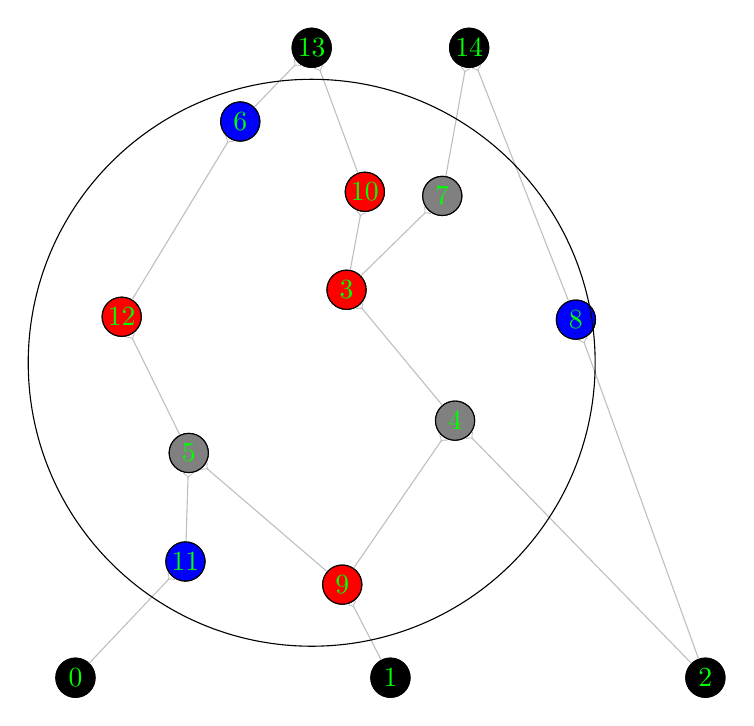
\begin{tikzpicture}[scale=4]
 \tikzset{
  nrn/.style={circle, draw, inner sep=5pt},
  con/.style={-<, gray!50}
 }
 \def\ni{3}
 \def\no{2}
 \def\nh{10}
 \pgfmathsetmacro{\total}{\ni+\nh+\no}
 \pgfmathsetmacro{\totalz}{\total-1}
%  \show\totalz
 \def\cp{.1}
 \pgfmathsetseed{16}
 
 \path [draw=none] (-1,-1) rectangle (1,1);
 
 \foreach \x [count=\i from 0] in {1,...,\ni} { \node [nrn] (\i) at ({(2*(\x-1)/(\ni-1))-1},-1) {}; }
 \foreach \x [count=\i from \ni] in {1,...,\nh} {
  \pgfmathsetmacro{\x}{-rand}
  \pgfmathsetmacro{\y}{.9*rand}
  \node [nrn] (\i) at (\x,\y) {};
 }
 \foreach \x [count=\i from \ni+\nh] in {1,...,\no} { \node [nrn] (\i) at ({(\x/\no)-.75},1) {}; }

%  \pgfmathsetmacro{\iend}{\ni+\nh-1}
%  \foreach \i in {1,...,20} {
%   \pgfmathsetmacro\src{int(random(0, \ni-1))}
%   \foreach \j in {1,...,10} {
%    \pgfmathsetmacro\dst{int(random(\src+1, \total-\no+1))}
%    \draw [con] (\src) -- (\dst);
% %    \node at (\i,\j) {\dst > \ni+\nh};
% %    \node at (1+.25*\i,1-.25*\j) {\src:\dst};
%    \xdef\src{\dst}
%    \ifnum \dst>\iend
%     \breakforeach
%    \fi
%   }
%  }

 \foreach \x [count=\i from 0] in {1,...,\ni} { \node at (\i) [nrn, fill=black] {}; }
 \pgfmathdeclarerandomlist{colors}{{gray}{red}{blue}}
 \foreach \x [count=\i from \ni] in {1,...,\nh} { 
  \pgfmathrandomitem{\color}{colors}
  \node at (\i) [nrn, fill=\color] {};
 }
 \foreach \x [count=\i from \ni+\nh] in {1,...,\no} { \node at (\i) [nrn, fill=black] {}; }
 
 \foreach \src/\dst in {0/11, 11/5, 5/12, 12/6, 6/13,
                        1/9, 9/5, 9/4, 4/3, 3/10, 10/13, 3/7, 7/14,
                        2/4, 2/8, 8/14}
  { \draw [con] (\src) -- (\dst); }
 
 \foreach \i in {0,...,\totalz} { \node [green] at (\i) {\i}; }
 
 \draw (-.25,0) circle (.9);
\end{tikzpicture}
\end{document}
